\chapter{Website}

The website is based on the Spring technologie,  it follow the MVC rule (Model-View-Controler). the view is separated from the controller and the model.

\begin{itemize}  
\item The view are the static web pages, in HTML and CSS, with pebble there are in .twig files
\item The controllers are files, coded in Java, which send data to the view
\item The model is like a kernel, he stock the informations, process them...

\end{itemize}  

Here is a schematic representation of the website architecture

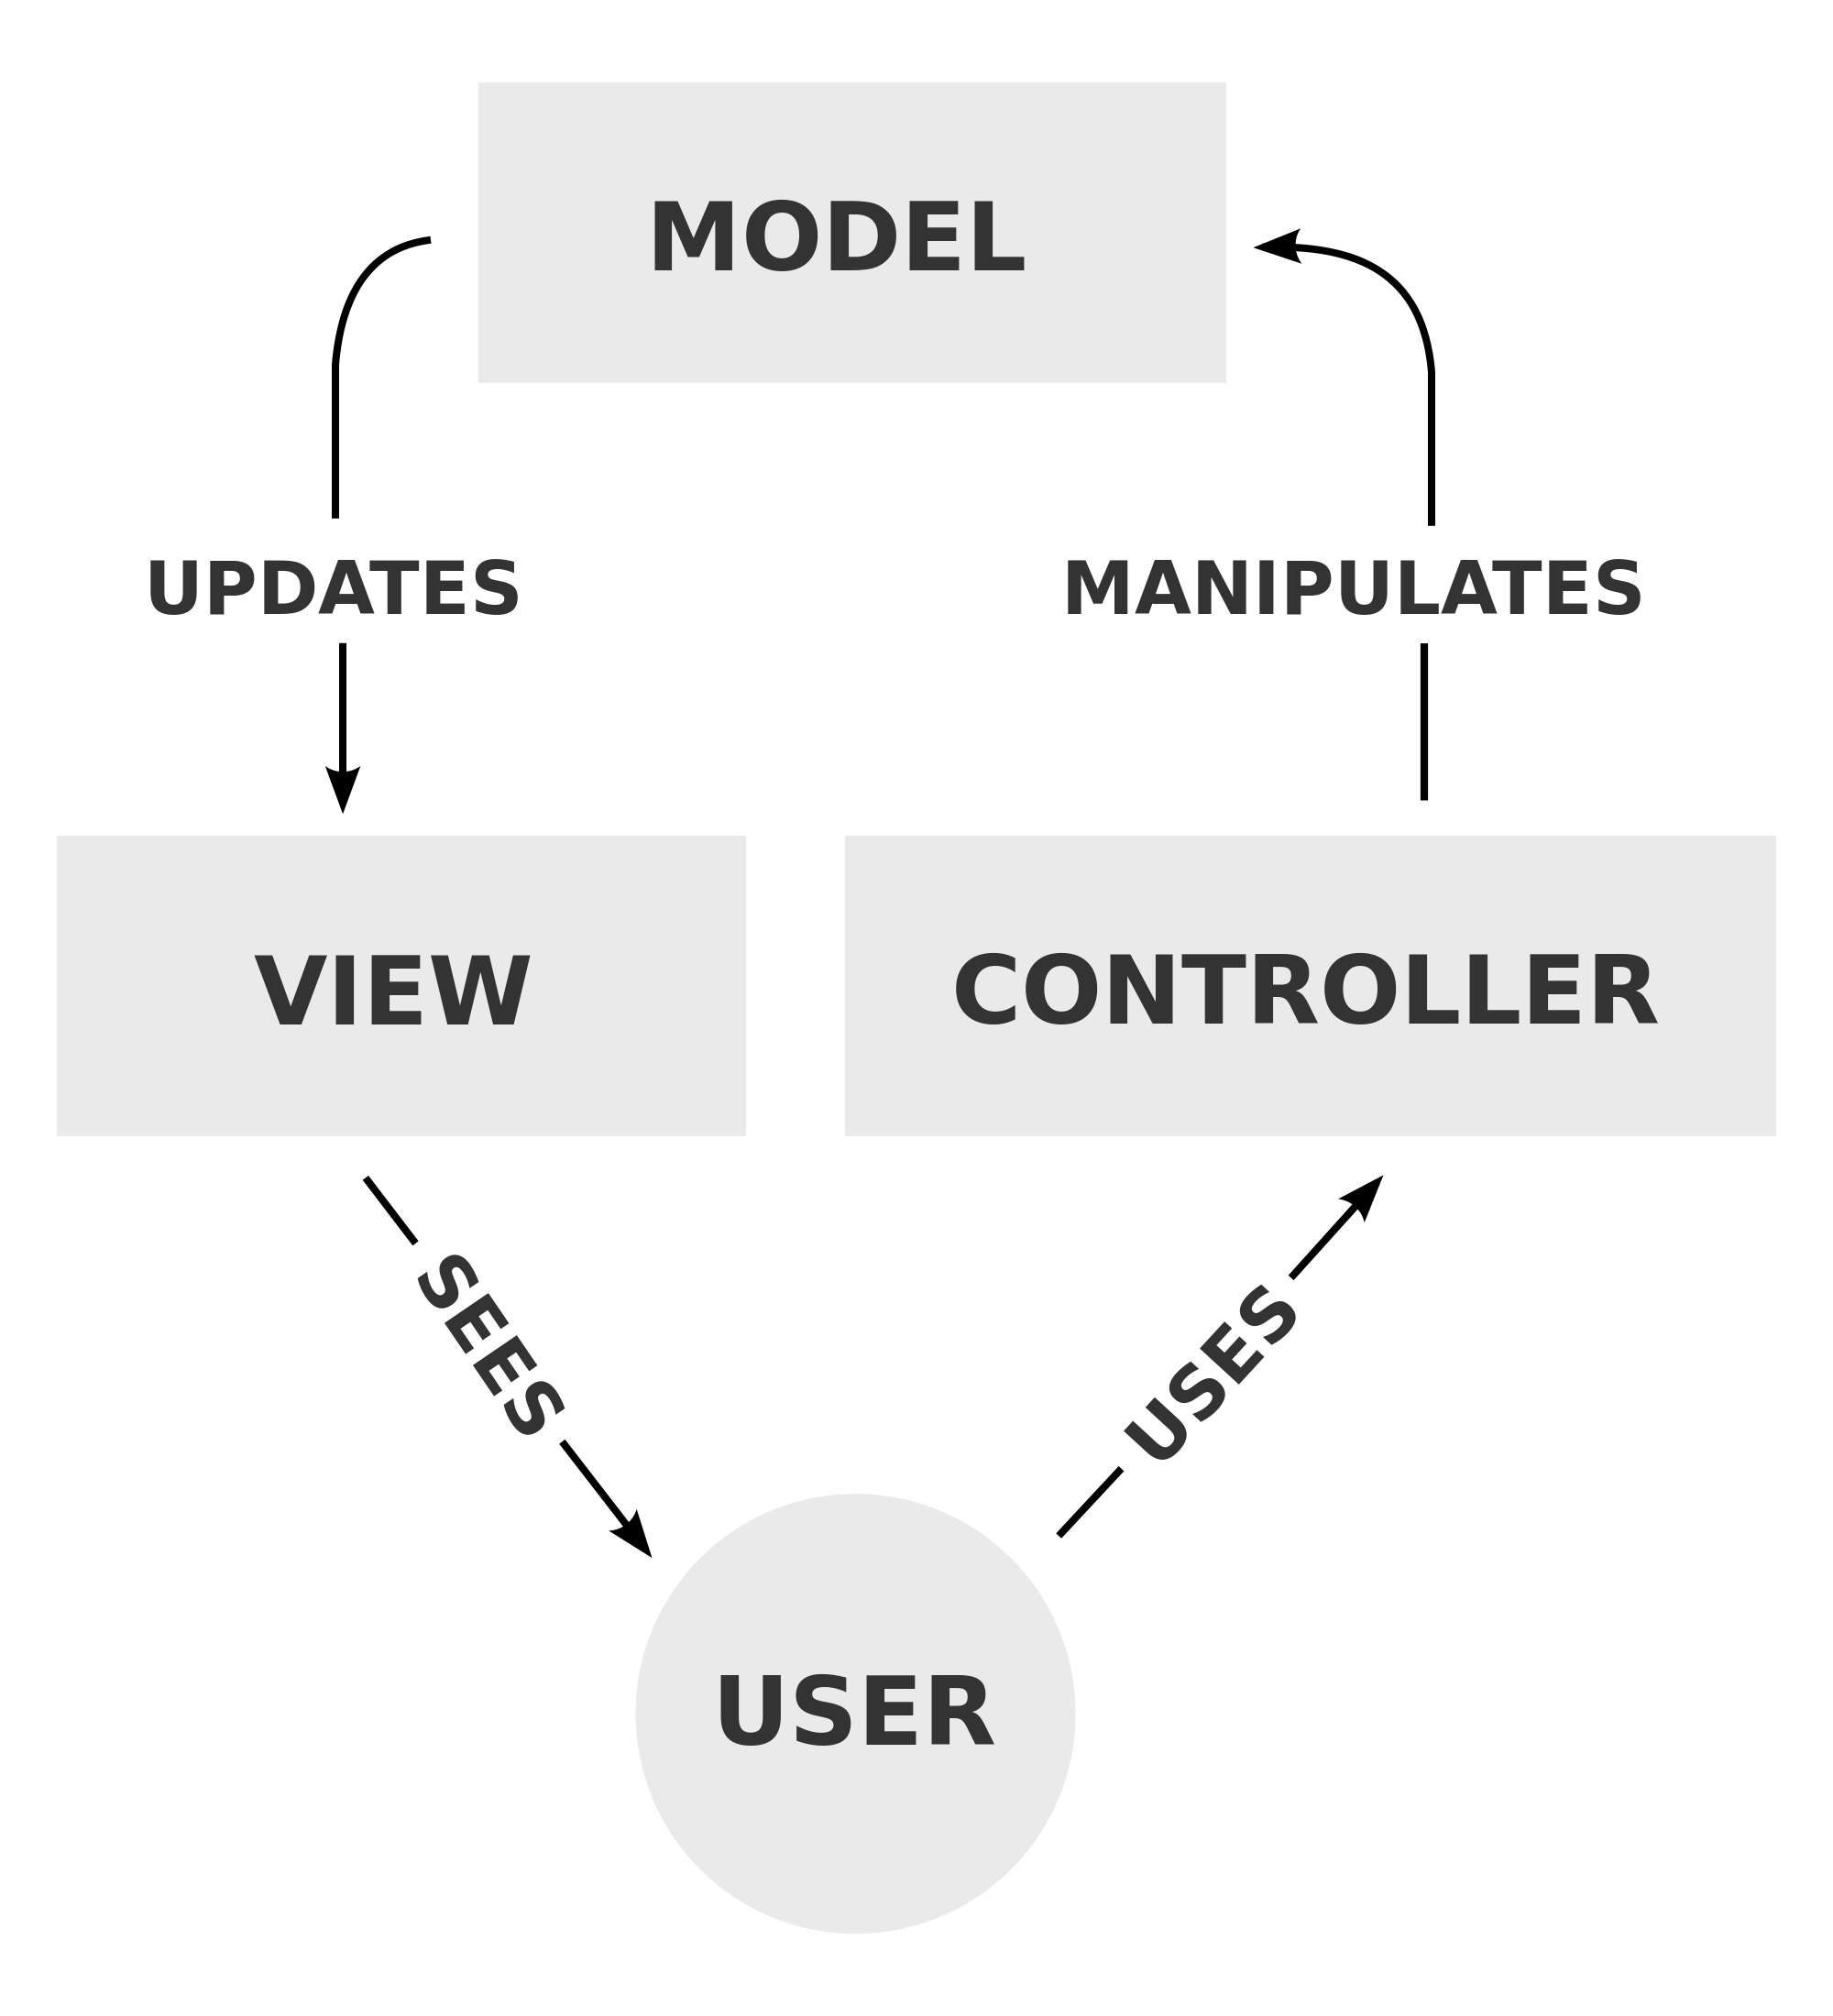
\includegraphics[width=0.50\textwidth]{img/mvc.png}



\section{DAO}

The DAO are the link between the program and the database. There are managed by the Hibernate technologie, coded in java.
In fact, we have one DAO per entity (switchboard, company...), those files contains functions which returns informations from the database.


\section{.twig}

The .twig files are an evolution of the HTML files, there are managed by pebble and represents the view of the website.
A .twig file can represent a file, or a part of a file (a layout), like a that we don't have to code every time the same code (like the menu...)